
\documentclass[10pt]{beamer}

\title[An Agile Omnidirectional Mobile Robot]{An Agile Omnidirectional Mobile Robot for Outdoor Usage}

\author[Li, Liu, et al.]{Zhuolun Li\inst{1} \and Xin Liu\inst{1} \and Zhiyang Qiang\inst{1} \\ Xiyu Zhu\inst{2} \and Angye Xie\inst{2}}
\institute[MEE, Sustech]{
\inst{1}
Robot Mobility and Manipulation Lab(ROMA), Sustech
\and
\inst{2}
Micro-Bio Robotics and Systems Lab, Sustech
}

\date{October 2021}

\logo{
\includegraphics[height=1cm]{photos/校徽.png}}

\usepackage{amsmath,amssymb,enumerate,epsfig,bbm,calc,color,ifthen,capt-of,multimedia,hyperref}
\usepackage{graphicx}
\usepackage{bibentry}

\usetheme{Boadilla}
\usecolortheme{beaver}

%%%% begin of slides
\begin{document}

\frame{\titlepage}
\begin{frame} % 什么是移动机器人?
\frametitle{Background}

\begin{columns}
\column{0.5\textwidth}
\begin{figure}
    \centering
    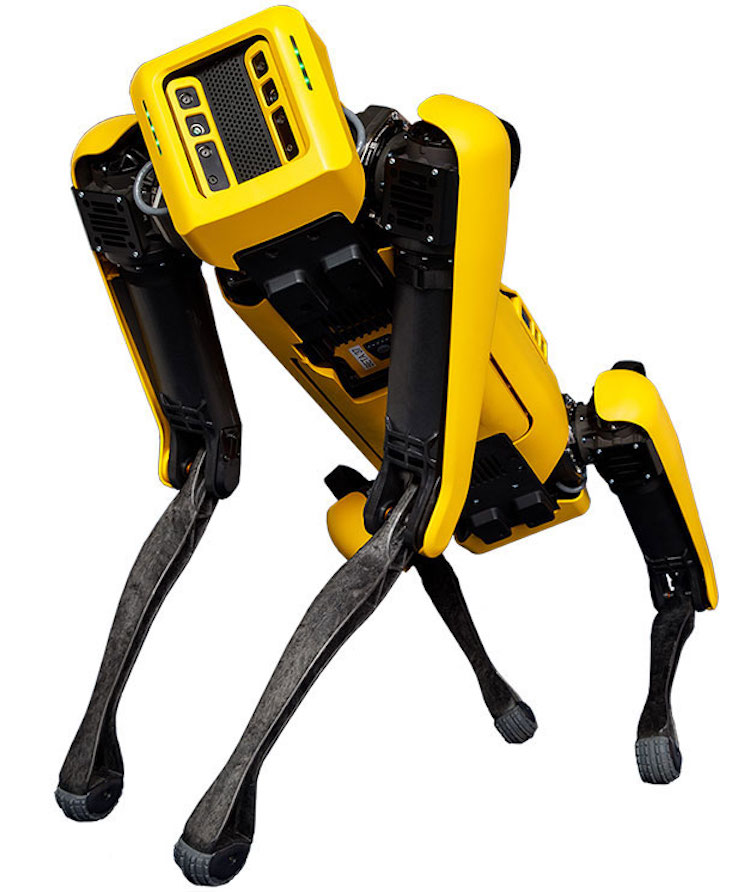
\includegraphics[width=2cm]{photos/boston-dynamics-spot.jpg} 
    \vspace{-0.3cm}
    \caption{Spot from Boston Dynamics}
    \label{fig:spot}
    \vspace{-0.7cm}
\end{figure}

\begin{figure}
    \centering
    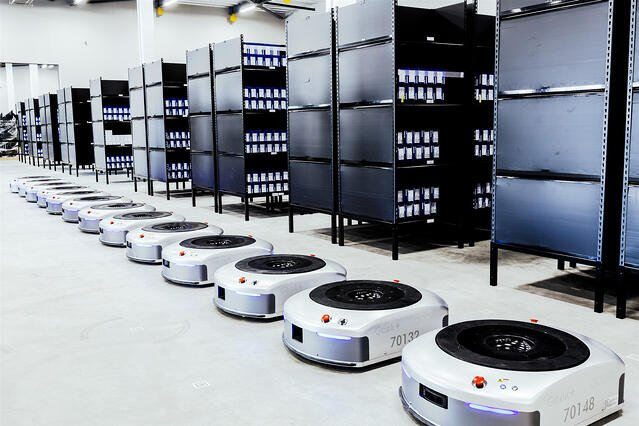
\includegraphics[width=3.2cm]{photos/Geek+ Picking.jpg}
    \vspace{-0.3cm}
    \caption{AGV from Geek+}
    \vspace{-0.7cm}
    \label{fig:geekplus}
\end{figure}

\begin{figure}
    \centering
    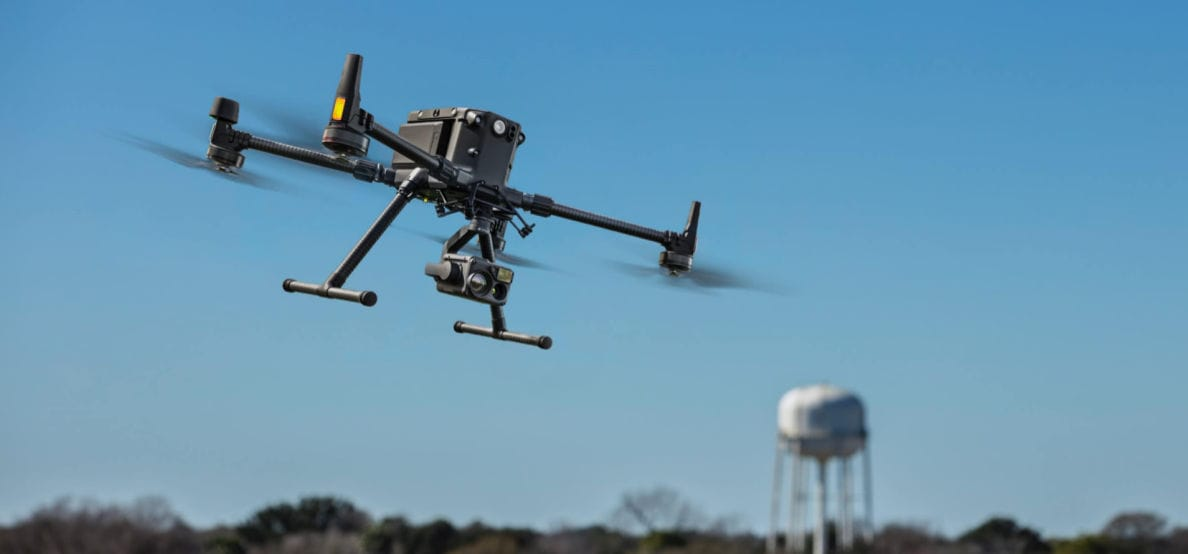
\includegraphics[width=3.2cm]{photos/dji.jpg}
    \vspace{-0.3cm}
    \caption{Quadrotor from DJI}
    \label{fig:grass}
\end{figure}

\column{0.5\textwidth}
% 什么是移动机器人?

\textbf{What is a mobile robot?}
\begin{itemize}
    \item A robot that can move itself to point A from point B. 
\end{itemize}

\textbf{Many mobile robots have been developed, it can be divided into: }
\begin{itemize}
    \item Legged mobile robots
    \item Wheeled mobile robots
    \item Aerial mobile robots
    \item ...
\end{itemize}
\end{columns}
\end{frame}

\begin{frame} % 移动机器人所处的环境是怎么样的?
\frametitle{Background}
\begin{columns}
\column{0.5\textwidth}
\begin{figure}
    \centering
    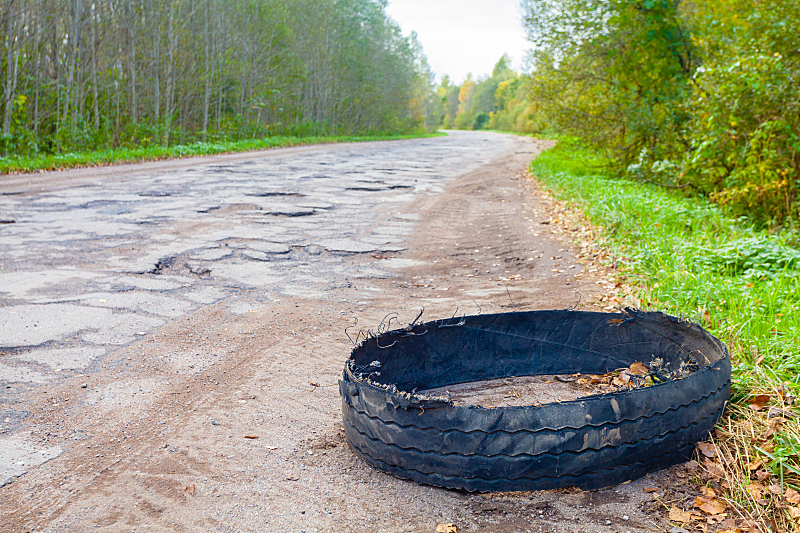
\includegraphics[width=4.6cm]{photos/rough-terrain.jpg} 
    \vspace{-0.3cm}
    \caption{Rough road}
    \label{fig:rough-terrain}
    \vspace{-0.7cm}
\end{figure}

\begin{figure}
    \centering
    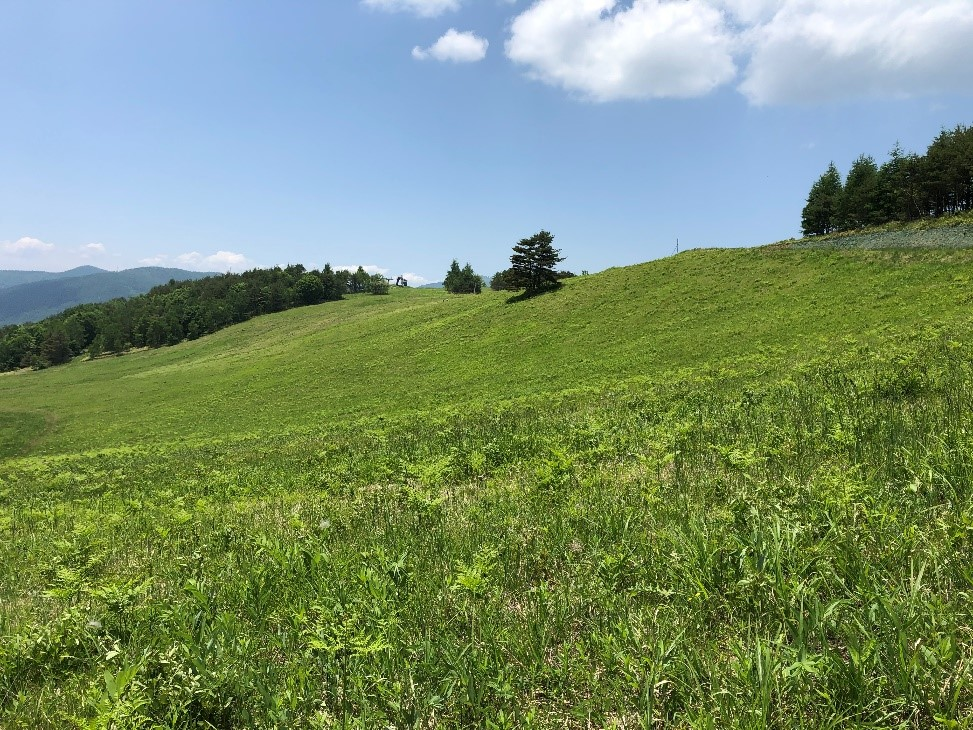
\includegraphics[width=4.6cm]{photos/草地.png}
    \vspace{-0.3cm}
    \caption{Grassland}
    \label{fig:grass-road}
\end{figure}

\column{0.5\textwidth}
\textbf{Road characteristics:}
% 特点:有一定的崎岖路面(可通过的障碍高度<15cm)、hard、
\begin{itemize}
    \item Rough \\(Obstacle height $<$ 15cm)
    \item Hard
    \item Not smooth
\end{itemize}
\textbf{Mobility requirements for a ground mobile robot in outdoors:}
% 移动能力、越障能力
\begin{itemize}
    \item Overcome complex environments
    \item Maintain stability
    \item Agile locomotion ($>1 body/s$) \\(Complete tasks on time)
\end{itemize}
\end{columns}
\end{frame}
\begin{frame} % Focus
\frametitle{Focus}
\centering
\textbf{Which mobile robots can meet these requirements?}
\end{frame}

\begin{frame} % 相关工作(腿式)
\frametitle{Related Work}
\begin{columns}
\column{0.5\textwidth}
\textbf{Legged mobile robots:}

\begin{itemize}
    \item Advantages
    \begin{itemize}
        \item Suitable for uneven terrain
        \item Agile mobility
    \end{itemize}
    \item Disadvantages
    \begin{itemize}
        \item Weak load capacity
        \item High power
        \item Unable to turn flexibly
    \end{itemize}
\end{itemize}

\column{0.5\textwidth}
\begin{figure}
    \centering
    \vspace{-1.2cm}
    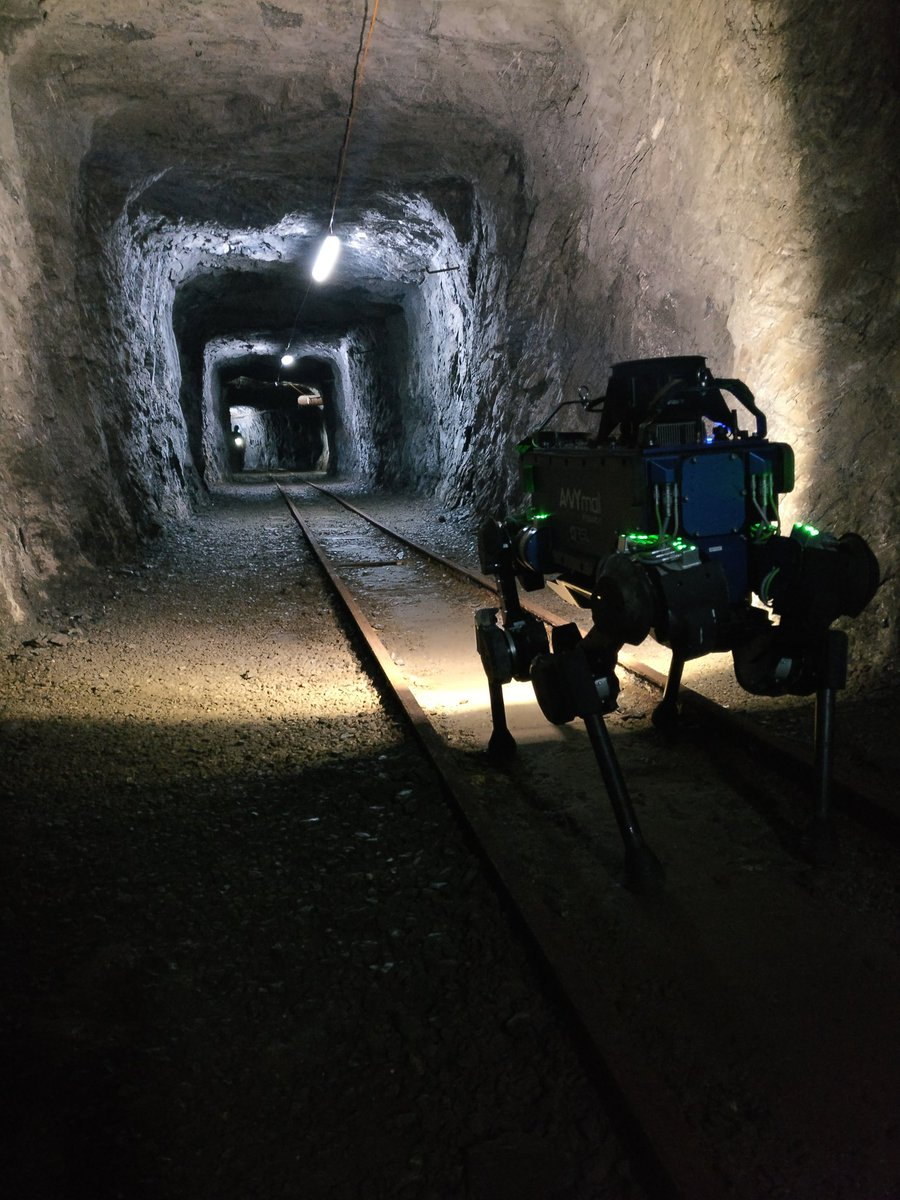
\includegraphics[width=4.5cm]{photos/qua-leg.png} 
    \vspace{-0.3cm}
    \caption{Anymal in Sub-T Challenge}
    \label{fig:sub-t}
    \vspace{-0.7cm}
\end{figure}
\end{columns}
\end{frame}

\begin{frame} % 相关工作(轮式)
\frametitle{Related Work}
\begin{columns}
\column{0.5\textwidth}
\textbf{Wheeled omni-directional mobile robots:}

\begin{itemize}
    \item Advantages
    \begin{itemize}
        \item Strong load capacity
        \item Agile omni-directional mobility
    \end{itemize}
    \item Disadvantages
    \begin{itemize}
        \item Not feasible for outdoor usage (Mecanum)
        \item Unable to steer rapidly (4WS-4WD)
    \end{itemize}
\end{itemize}

\column{0.5\textwidth}
\begin{figure}
    \centering
    \vspace{-1.2cm}
    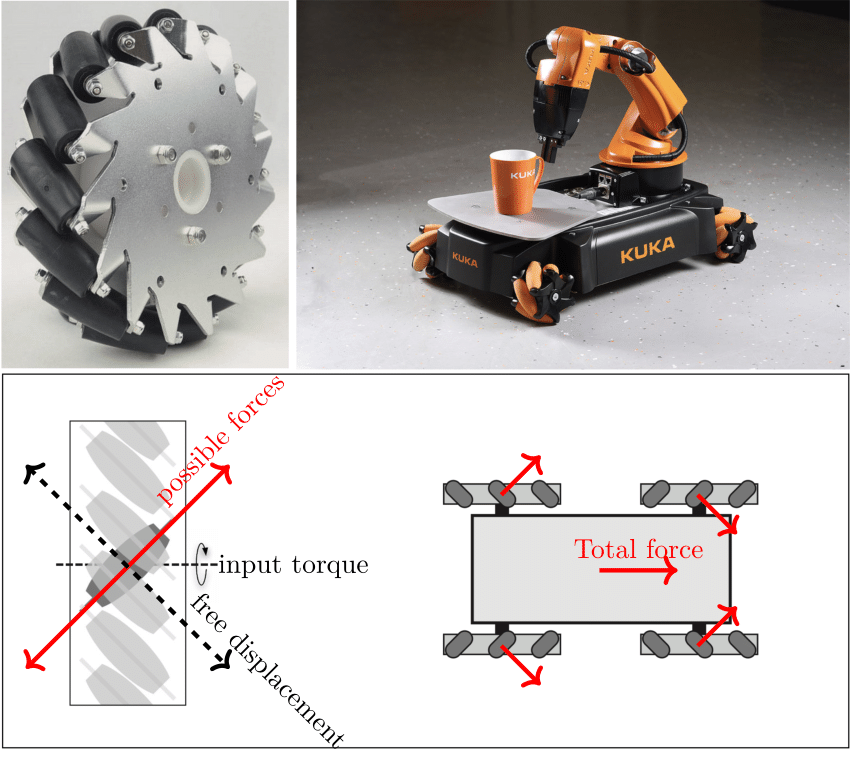
\includegraphics[width=4cm]{photos/mecanum.png} 
    \vspace{-0.3cm}
    \caption{Youbot from KUKA}
    \label{fig:Macanum}
    \vspace{-0.7cm}
\end{figure}

\begin{figure}
    \centering
    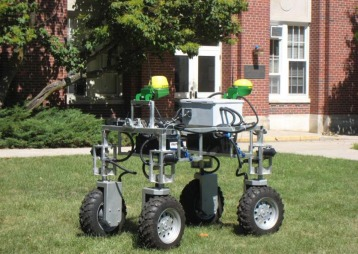
\includegraphics[width=4cm]{photos/4WS-4Wd.png} 
    \vspace{-0.3cm}
    \caption{4WS-4WD robot}
    \label{fig:4ws-4wd}
    \vspace{-0.7cm}
\end{figure}
\end{columns}
\end{frame}

\begin{frame} % 相关工作(轮腿混合)
% 轮式与足式的融合交叉发展 
% 腿-》轮   轮-》腿
\frametitle{Related Work}
\begin{columns}
\column{0.4\textwidth}
\textbf{Wheel-legged mobile robots:}

\begin{itemize}
    \item Developed from wheeled robot: 
    \begin{itemize} 
        \item Add active joints to the body
    \end{itemize} 
    \item Developed from legged robot: 
    \begin{itemize} 
        \item Add wheels on joints
    \end{itemize} 
\end{itemize} 


\textbf{Robots still have some disadvantages!}

\column{0.55\textwidth}
\begin{figure}
    \centering
    \vspace{-1.2cm}
    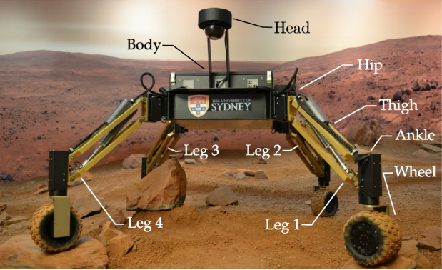
\includegraphics[width=4cm]{photos/wheel-leg.png} 
    \vspace{-0.3cm}
    \caption{Wheel-on-Leg Rover from KUYD}
    \label{fig:wheel-leg}
    \vspace{-0.3cm}
\end{figure}

\begin{figure}
    \centering
    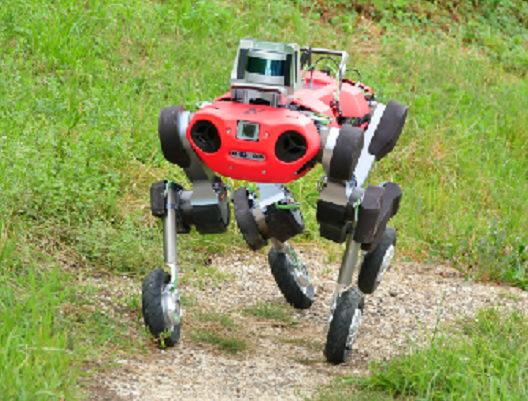
\includegraphics[width=4cm]{photos/anymal-1.png} 
    \vspace{-0.3cm}
    \caption{wheeled quadruped from ETH}
    \label{fig:anymal-1}
    \vspace{-0.7cm}
\end{figure}
\end{columns}
\end{frame}


\begin{frame}{Redefine the problem} 
    \centering
    \textbf{Can we design an omni-directional wheeled robot \\
    to meet these requirements?}
\end{frame}

% \begin{frame}{Solution}
    
% \end{frame}

\begin{frame}{Reference} 
\footnotesize{
\begin{thebibliography}{99}
[1] W. Reid, F. J. Pérez-Grau, A. H. Göktoğan and S. Sukkarieh, Actively articulated suspension for a wheel-on-leg rover operating on a Martian analog surface, 2016 IEEE International Conference on Robotics and Automation (ICRA), 2016.
\end{thebibliography}

\begin{thebibliography}{99}
[2] Y. Xu, J. Tu, G. Tang, Robust navigation control of a 4WD/4WS agricultural robotic vehicle, Computers and Electronics in Agriculture, Volume 164, 2019.
\end{thebibliography}

\begin{thebibliography}{99}
[3] M. Bjelonic et al., "Keep Rollin’—Whole-Body Motion Control and Planning for Wheeled Quadrupedal Robots," in IEEE Robotics and Automation Letters, vol. 4, no. 2, pp. 2116-2123, April 2019.
\end{thebibliography}
}

\end{frame}

\begin{frame}{End} 
    \centering
    \textbf{Thanks For Your Listening! \\ Q\&A}
\end{frame}




% \begin{frame}{Solution} 
% \begin{columns}
% \column{0.5\textwidth}
    
% \column{0.5\textwidth}
% \begin{figure}
%     \centering
%     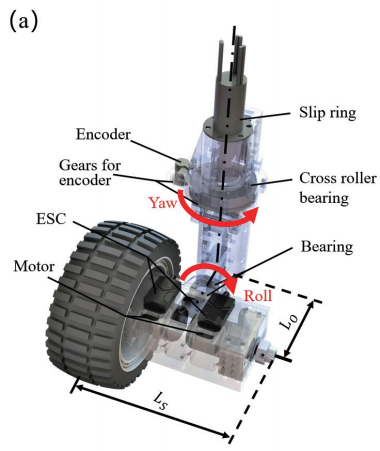
\includegraphics[width=4cm]{photos/ASOC_module.png} 
%     \vspace{-0.3cm}
%     \caption{ASOC module}
%     \label{fig:mine}
%     \vspace{-0.7cm}
% \end{figure}
% \end{columns}
% \end{frame}

\end{document}

 
% 欠缺点:
% 对性能的定义,数据性的指标。
% 潜在问题的排除,定义scope,排除负载能力和天气部分。
% 留伏笔,讲一下下次要讲什么。
% 对具体技术的分析。
% 与研究阶段的东西做对比